\documentclass[conference]{IEEEtran}
\IEEEoverridecommandlockouts
% The preceding line is only needed to identify funding in the first footnote. If that is unneeded, please comment it out.
%Template version as of 6/27/2024

\usepackage{cite}
\usepackage{amsmath,amssymb,amsfonts}
\usepackage{graphicx}
\usepackage{textcomp}
\usepackage{xcolor}
\def\BibTeX{{\rm B\kern-.05em{\sc i\kern-.025em b}\kern-.08em
    T\kern-.1667em\lower.7ex\hbox{E}\kern-.125emX}}
\begin{document}

\title{Reconstructing Axially Symmetric 3D Pottery Using Genetic Algorithms}

\author{\IEEEauthorblockN{Taha Zahid, Zain Naqi, Sheikh Muhammad Sufyan, Saleha Raza}
\IEEEauthorblockA{\textit{Dhanani School of Science and Engineering} \\
\textit{Habib University}\\
Karachi, Pakistan \\
\{tz09220, zn09224, ss09215\}@st.habib.edu.pk \quad saleha.raza@sse.habib.edu.pk}
}

\maketitle

\begin{abstract}
The computational reassembly of broken archaeological pottery is a combinatorial challenge due to the large search space and geometric ambiguity from thin fracture surfaces. Existing methods rely on greedy incremental search or data-driven learning, each with limitations in scalability or generalization. We present a genetic algorithm (GA) system for 3D pottery reassembly, targeting the reconstruction of individual axially symmetric pots from their constituent sherds. Building on the Structure-from-Sherds++ (SfS++) pipeline, we replace the BAISER beam search with a population-based evolutionary search while preserving the geometric feature extraction and pairwise matching stages. Our GA uses an integer chromosome representation over precomputed match candidates, a shard-partition crossover operator, shard-centric mutation, and a multi-component fitness function combining match quality, cycle consistency, edge and rotation residual penalties, connectivity rewards, and voxel-based collision detection. Experiments on the SfS++ benchmark dataset show that our approach achieves results comparable to SfS++ on some pots while lagging on others, showing the feasibility of evolutionary search and identifying areas for improvement. We further present convergence analysis and visual reconstruction progression to show how the evolutionary search builds up assemblies over time.
\end{abstract}

\begin{IEEEkeywords}
genetic algorithm, pottery reassembly, evolutionary computation, 3D reconstruction, archaeological fragment assembly, fitness function design, combinatorial optimization
\end{IEEEkeywords}

\section{Introduction}
The reassembly of broken pottery recovered from archaeological sites remains a longstanding challenge in archaeology. Studying these artifacts is essential for understanding the societies that once inhabited these sites. However, even skilled archaeologists and restoration experts with knowledge of historical context and geometric structure face a tedious and time-consuming process, often requiring days to reconstruct a single pottery \cite{b1}.

This raises the need for computer-driven methods that can solve this problem more efficiently and in significantly less time. By nature, this is a combinatorial problem: even a single pottery broken into 10 pieces can have 3,628,800 possible arrangements, not accounting for the rotational and translational degrees of freedom of each fragment. Over the past few years, significant research has been dedicated to this task, one branch of which focuses on axially symmetric potteries \cite{b2}.

Existing approaches to this problem range from geometric feature matching to deep learning and parallel search methods, each with limitations in scalability, data requirements, or computational cost \cite{b1}. Among the most successful recent methods is Structure-from-Sherds++ (SfS++) \cite{b2}, which draws inspiration from incremental Structure-from-Motion pipelines. SfS++ extracts axis-based geometric features and breakline descriptors from each sherd, performs pairwise matching using the Longest Common Subsequence (LCS) algorithm, and then assembles the pot incrementally using a multi-graph beam search technique called BAISER (Base-Agnostic Incremental ShErd Registration). SfS++ achieves state-of-the-art results on real pottery datasets, including the task of simultaneously reconstructing multiple pots from mixed fragment collections.

In this paper, we focus on reconstructing individual axially symmetric pots where all sherds belong to the same vessel. We build on the SfS++ pipeline, preserving its feature extraction and pairwise matching stages, and replace the BAISER beam search with a genetic algorithm. We present a GA-based solution for 3D pottery reassembly and analyze its reconstruction accuracy and computational cost.

\section{Literature Review}
\subsection{Geometric Feature Matching Approaches}
A standard computational pipeline for reassembly begins with surface segmentation, where algorithms distinguish a sherd’s intact exterior from its fractured surfaces using either intrinsic geometric properties or learning-based techniques. Following segmentation, pairwise matching methods utilize geometric descriptors or boundary curves extracted from fracture surfaces to estimate the relative rigid alignment between complementary sherds \cite{b1}, \cite{b3}.

Huang et al. \cite{b4} present a system for automatic digital reassembly of broken 3D objects using only the geometric properties of fragments. Unlike earlier methods that required nearly flat pieces or perfect matches, their pipeline handles fragments with arbitrary, irregular geometries and partial matches. Notably, they introduce a multi-piece matching approach that aligns all fragments simultaneously, preventing the compounding errors that arise when pieces are joined one at a time.

Winkelbach and Wahl \cite{b5} propose a surface matching method for reassembling broken 3D solids. They use a hierarchical cluster tree of oriented points rather than relying on surface features or requiring an initial pose estimate. The method systematically searches the full space of possible contact poses through a simultaneous depth-first traversal of both fragments’ cluster trees. The method further prunes hypotheses whose upper-bound contact quality falls below the best match found so far. The approach guarantees termination and returns the globally optimal pose, achieving accurate alignments in under nine seconds across diverse test cases. However, it addresses only pairwise matching and does not scale to the full multi-fragment reassembly problem.

Papaioannou et al. \cite{b6} extend this direction by combining fracture surface matching with salient features extracted from the intact sides of fragments, making the approach more robust when fracture surfaces alone are insufficient for reliable alignment. Their pipeline further incorporates a symmetry-based completion step to recover missing geometry, producing a more complete restoration. However, approaches that rely purely on geometric matching still struggle in the presence of noise, missing fragments, and false positive matches, limiting their effectiveness in real-world scenarios \cite{b1}.

Gregor et al. \cite{b7} propose a broader automated pipeline for reconstructing defective cultural heritage artifacts. Their pipeline classifies surfaces to distinguish intact areas from fractured edges using Heat Kernel Signatures, a geometric descriptor robust to damage and deformation, before performing reassembly, symmetry-based completion, and inpainting in sequence. For axially symmetric pottery in particular, rotational symmetry plays a critical role in guiding reassembly by heavily constraining the search space \cite{b1}. However, their pipeline is designed as a general cultural heritage restoration tool rather than one tailored to pottery reassembly specifically.

Pintus et al. \cite{b8} survey geometric analysis techniques in cultural heritage, organizing the field by geometric scale and object cardinality. They identify pottery reconstruction as a domain that benefits from axial symmetry. They further note that the multi-fragment assembly problem, framed as a scalable and globally optimal combinatorial search, remains an open challenge. Their taxonomy shows that no existing approach combines population-based search with domain-specific symmetry constraints for 3D pottery.

\subsection{Data-Driven and Deep Learning Approaches}
Some approaches use deep learning techniques to train convolutional neural networks (CNNs) on the fragment’s geometry. These data-driven methods require significant amounts of well-labeled training data and long training times, posing practical challenges in archaeological settings where labeled data is scarce \cite{b1}.

Pinho et al. \cite{b9} propose PotNet, a 1D convolutional neural network that predicts the rotation and translation required to place a sherd’s point cloud into its correct position within the original vessel’s coordinate system. To address the scarcity of real-world training data, the method relies on synthetically generated fragments produced by virtually shattering complete vessel models. Evaluated on both synthetic fragments and real-world scanned sherds, PotNet achieves average positioning errors in the centimeter range with millimeter-level standard deviations. Rather than producing a final reconstruction directly, it narrows the search space by providing a strong initial position estimate, which is subsequently refined by classical algorithms such as Iterative Closest Point (ICP). While promising, this approach inherits the general limitations of data-driven methods: its accuracy depends on the quality and diversity of synthetic training data, and generalization to unseen vessel shapes or fragment types remains a challenge.

\subsection{Parallel Search Approaches}
Other approaches rely on parallelism, constructing a search tree with multiple branches explored simultaneously to find the best possible reconstruction. While thorough, these methods require substantial computational resources and significant runtime \cite{b1}. A notable example is the BAISER beam search technique employed by Yoo et al. \cite{b2}, which focuses on axially symmetric pottery and is the foundation of our work.

\subsection{Genetic Algorithms for Reconstruction}
Genetic algorithms have been successfully applied to 2D reconstruction problems, demonstrating their ability to navigate large combinatorial search spaces without committing to early greedy decisions.

Sholomon et al. \cite{b10} propose the first effective genetic algorithm-based jigsaw puzzle solver. Their core contribution is a crossover procedure that merges two parent solutions into an improved child by detecting, extracting, and combining correctly assembled segments, an approach grounded in the best-buddy similarity metric, which identifies pairs of puzzle pieces that are mutually the best match for each other along a given edge. Their solver achieved state-of-the-art performance on puzzles of sizes previously unattempted.

Building on this, Sholomon et al. \cite{b11} extend their solver to handle puzzles with unknown dimensions and unknown piece orientation, successfully reconstructing a puzzle of 22,755 pieces. Their solver also shows the ability to simultaneously reconstruct a mixed bag of 16,405 pieces drawn from seven different images, showing the scalability of genetic approaches to large and ambiguous reassembly problems.

Sizikova and Funkhouser \cite{b12} address the global assembly of 2D fragmented wall paintings suffering from missing pieces and severe erosion. Traditional greedy methods fail on such artifacts because early incorrect matches propagate errors irreversibly. Their unsupervised genetic algorithm instead maintains a diverse population of partial reconstructions, evaluating clusters via a fitness function that rewards dense match connections and geometrically sound convex hulls. This work is of relevance to our approach, as it shows the feasibility of genetic algorithms for noisy, real-world fragment reassembly.

To our knowledge, no prior work has applied genetic algorithms to 3D pottery reassembly, leaving this a largely unexplored direction that we address in this paper.

\section{Methodology}
\subsection{Problem Formulation}
The problem consists of two subproblems: (i) geometric feature extraction and matching of sherds, and (ii) the reassembly process itself \cite{b1}.

Let $\mathcal{S} = \{s_1, s_2, \ldots, s_n\}$ denote the set of $n$ pottery sherds, each represented as a 3D point cloud with associated surface normals. The goal is to find a set of rigid transforms $\{T_1, T_2, \ldots, T_n\}$ and a connection graph $G$ over $\mathcal{S}$ such that the assembled configuration maximally reconstructs the original vessel. Each edge $(i, j)$ in $G$ represents a physical contact between sherds $s_i$ and $s_j$, with an associated relative transform $T_{ij}$.

Following SfS++ \cite{b2}, we restrict our focus to axially symmetric pottery, where rotational symmetry about the vertical axis substantially constrains the search space. Each shard has a breakline $B_i$ extracted from its fracture surface, and pairwise matching hypotheses are generated by the Longest Common Subsequence (LCS) algorithm on these breaklines.

\subsection{Pipeline Overview}
Our system preserves the geometric preprocessing stages of SfS++ intact and replaces only the BAISER beam search with a GA. The full pipeline is:
\begin{enumerate}
    \item \textbf{Feature extraction:} Axis estimation, breakline extraction, and rim segmentation per sherd.
    \item \textbf{Pairwise matching:} LCS-based matching produces a candidate pool $\mathcal{M}$ of pairwise match hypotheses, each carrying a transform, inlier count, and score.
    \item \textbf{Pairwise pruning:} Geometric consistency filtering reduces $|\mathcal{M}|$ to a tractable candidate set.
    \item \textbf{Pair group construction:} Candidates in $\mathcal{M}$ are grouped by shard pair, forming $\mathcal{G} = \{G_1, G_2, \ldots, G_m\}$ where each $G_k$ contains all match hypotheses between a specific pair of sherds.
    \item \textbf{GA search:} A population-based search over chromosomes encoding which pair groups to accept and which match hypothesis to select in the accepted pair groups.
    \item \textbf{Assembly decoding:} The best chromosome is decoded into global transforms via priority-queue BFS pose propagation, where the highest-confidence edges are expanded first.
\end{enumerate}

\subsection{Chromosome Representation}
A chromosome $\mathbf{c}$ is an integer vector of length $m = |\mathcal{G}|$, one gene per pair group. Gene $c_k \in \{0, 1, \ldots, |G_k|\}$ encodes the match selection decision for pair group $G_k$:
\begin{equation}
c_k =
\begin{cases}
0 & \text{reject all matches for this pair} \\
j & \text{accept the } j\text{-th match hypothesis in } G_k
\end{cases}
\end{equation}
This representation guarantees that at most one match between any pair of sherds is ever accepted, reflecting the physical constraint that two sherds can only fit together in one way. The chromosome length is fixed at $m$, enabling standard fixed-length crossover and mutation operators.

\subsection{Population Initialization}
Each chromosome is initialized by independently sampling each gene. Gene $c_k$ is set to 0 (reject) with probability $p_{\text{inactive}} = 0.05$. With the remaining probability of 0.95, a match hypothesis is selected using rank-based selection. To perform this selection, candidates within a pair group are ranked by their density score:
\begin{equation}
\text{density}(j) = \frac{\text{inlier}(j)}{1 + \text{score}(j)}
\end{equation}
Here, $\text{inlier}(j)$ is the number of breakline point correspondences that fall within a distance threshold during pairwise ICP registration; higher values indicate stronger geometric agreement between two sherds. $\text{score}(j)$ is the LCS dissimilarity metric produced by the pairwise matching stage; lower values indicate a better match. The density metric combines both signals: a high inlier count and low score yield a high density, identifying the most reliable match hypotheses.

Candidates are sorted by density in descending order, and linear rank weights are assigned (the best-ranked candidate receives the highest weight). Selection is then performed by roulette wheel on these rank weights:
\begin{equation}
w_{\text{rank}}(j) = |G_k| - \text{rank}(j), \quad P(\text{select } j) = \frac{w_{\text{rank}}(j)}{\sum_{j' \in G_k} w_{\text{rank}}(j')}
\end{equation}
This rank-based policy biases initialization toward higher-quality match hypotheses without being dominated by outlier density values.

\subsection{Fitness Function}
The fitness function $F(\mathbf{c})$ evaluates the geometric quality of the assembly encoded by chromosome $\mathbf{c}$. It combines six components:
\subsubsection{Match Quality Score} For each accepted match at gene $c_k > 0$, the quality contribution uses the density metric:
\begin{equation}
q_k = \frac{\text{inlier}(c_k)}{1 + \text{score}(c_k)}
\end{equation}
The total quality reward is $\sum_{k} q_k$.
\subsubsection{Connectivity Reward} Let $C_{\max}$ be the size of the largest connected component in the assembly graph induced by the chromosome. The connectivity reward encourages assembling more sherds into a single connected structure:
\begin{equation}
F_{\text{conn}} = \lambda_{\text{conn}} \cdot C_{\max}
\end{equation}
\subsubsection{Cycle Consistency Penalty} For every triangle $(a, b, c)$ of sherds where all three pairwise matches are accepted, the loop closure residual is:
\begin{equation}
\epsilon_{abc} = \|\mathbf{t}_{ab} \oplus \mathbf{t}_{bc} - \mathbf{t}_{ac}\|
\end{equation}
where $\mathbf{t}_{ij}$ is the translation component of the accepted transform between sherds $i$ and $j$, and $\oplus$ denotes transform composition. A penalty is accumulated for all triangles with $\epsilon_{abc} > \tau_{\text{cycle}} = 30.0$:
\begin{equation}
F_{\text{cycle}} = -2.0 \cdot \sum_{(a,b,c)} \max(0, \epsilon_{abc} - \tau_{\text{cycle}})
\end{equation}
This detects globally inconsistent assemblies that pairwise metrics miss.
\subsubsection{Edge and Rotation Residual Penalties} After BFS pose propagation from multiple roots, each shard receives a global pose. The BFS-propagated relative transform between sherds $a$ and $b$ is $\hat{T}_{ab} = T_b^{-1}T_a$, derived by composing transforms along the BFS tree. The pairwise transform $T_{ab}$ is the direct transform stored in the accepted match hypothesis from the LCS matching stage. When there are multiple paths between two sherds, BFS may accumulate errors along longer paths, and the residual measures this inconsistency:
\begin{equation}
r_{ab}^{t} = \|\hat{\mathbf{t}}_{ab} - \mathbf{t}_{ab}\|, \quad F_{\text{res}}^{t} = -\lambda_r \sum_{(a,b)} \max(0, r_{ab}^{t} - \tau_r)^2
\end{equation}
The rotation residual uses the matrix logarithm of $\hat{R}_{ab}R_{ab}^{-1}$ to extract the rotation angle:
\begin{equation}
F_{\text{res}}^{r} = -\lambda_r^{\text{rot}} \sum_{(a,b)} \max(0, r_{ab}^{r} - \tau_r^{\text{rot}})
\end{equation}
For each edge, only the maximum residual across all BFS roots is retained, to avoid double-penalizing large assemblies for the same inconsistency.
\subsubsection{Overlap Penalty} After BFS pose propagation, the global positions of all placed sherds are known. The overlap penalty checks all pairs of sherds within each connected component to detect physically implausible interpenetration.
The collision cloud for each shard is precomputed as follows: surface points (both inner and outer surfaces) are collected, points within 2.0 mm of the breakline edges are excluded to avoid penalizing legitimate contact regions, and the remaining points are voxel-downsampled to a 5.0 mm grid, retaining one representative point per voxel cell. A kd-tree is built on each shard’s collision cloud for efficient nearest-neighbor queries.

For a pair of placed sherds $(i, j)$, each point in shard $i$'s collision cloud is transformed to global space and its nearest neighbor in shard $j$'s cloud is found via the kd-tree. A ``hit'' is registered when the nearest-neighbor distance is within $\epsilon_{\text{coll}} = 2.5$ mm. The penalty combines the hit ratio (fraction of query points that produce hits), the average penetration depth, and a saturation function to produce a bounded overlap score per pair:
\begin{equation}
F_{\text{overlap}} = -\lambda_{\text{overlap}} \sum_{(i,j)} f_{\text{overlap}}(i, j)
\end{equation}
where $f_{\text{overlap}}(i, j)$ is the overlap score combining hit ratio and depth information, and $\lambda_{\text{overlap}} = 1200.0$.

The full fitness function is:
\begin{equation}
F(\mathbf{c}) = \sum_{k} q_k + F_{\text{conn}} + F_{\text{cycle}} + F_{\text{res}}^{t} + F_{\text{res}}^{r} + F_{\text{overlap}}
\end{equation}

\subsection{Assembly Decoding via Priority-Queue BFS}
The accepted matches define a connection graph. To decode a chromosome into global shard poses, we use a priority-queue-based BFS expansion similar to Prim’s minimum spanning tree algorithm. Starting from the first valid shard, the frontier is maintained as a max-priority queue ordered by edge weight (inlier count). At each step, the highest-confidence unvisited edge is expanded:
\begin{equation}
T_{\text{next}} = T_{\text{current}} \cdot T_{\text{current}\to\text{next}}
\end{equation}
This ensures that the most reliable pairwise transforms are used first when building the pose tree, reducing error accumulation along the BFS paths.

\subsection{Genetic Operators}
\subsubsection{Selection} Tournament selection with tournament size 3 is used. Three chromosomes are drawn uniformly at random and the one with the highest fitness is returned as a parent. This provides moderate selection pressure while maintaining population diversity.
\subsubsection{Crossover} We use a shard-partition crossover operator. Each shard is randomly assigned to one of two parents with equal probability. For each pair group gene $c_k$ corresponding to sherds $(x, y)$:
\begin{itemize}
    \item If both sherds $x$ and $y$ are assigned to the same parent, the child inherits that parent’s gene value for $c_k$.
    \item If the sherds are split between parents, the child inherits from either parent with equal probability (0.5 each).
\end{itemize}
This crossover preserves locally consistent sub-assemblies: when both sherds of a pair belong to the same parent, their relationship is inherited intact rather than being disrupted by a random crossover point.
\subsubsection{Mutation} Mutation uses a shard-centric strategy with probability $p_m = 0.10$. When triggered, a random shard is selected, and one of its incident pair group genes is chosen uniformly at random. The gene is then either deactivated (set to 0) with 50\% probability or re-sampled via the rank-based selection procedure described in population initialization with the remaining 50\% probability. This shard-centric approach focuses mutation on a specific shard’s relationships, producing more targeted exploration than independent per-gene mutation.
\subsubsection{Elitism} The top $e = 6$ chromosomes are preserved directly into the next generation without modification, ensuring the best solution found is never lost.

\section{Experimental Setup}
\subsection{Dataset}
We evaluate on the SfS++ benchmark dataset \cite{b2}, which contains 3D scanned pottery sherds from ten different archaeological pots. We evaluated our system on seven of these pots (A, B, C, F, G, H, and J). We omitted Pots D, E, and I due to high computational cost making it infeasible for our current hardware. Each sherd is represented as a point cloud with surface normals, breakline points, and rim segmentation. The ground truth graph $G^*$ and transforms $\{T_i^*\}$ are used to compute accuracy metrics.

\subsection{Evaluation Metrics}
We report the standard SfS++ accuracy metrics:
\begin{itemize}
    \item \textbf{Sherd Accuracy (SA):} The percentage of correctly placed sherds over the total number of sherds. A sherd is considered correctly placed if at least one of its edges is placed correctly within a rotation threshold and translation threshold of the ground truth transform.
    \item \textbf{Edge Accuracy (EA):} The percentage of correctly identified pairwise connections over the total number of ground truth connections across the entire assembly.
\end{itemize}

\subsection{Baseline}
We compare against the BAISER beam search of SfS++ \cite{b2} run on identical input (same pairwise matches after pruning). Since both methods share the feature extraction and matching stages, any performance difference is attributable solely to the search algorithm.

\subsection{Hyperparameters}
Table \ref{tab1} lists all GA hyperparameters used in our experiments.

\begin{table}[htbp]
\caption{GA Hyperparameters}
\begin{center}
\begin{tabular}{|l|l|l|}
\hline
\textbf{Parameter} & \textbf{Value} & \textbf{Rationale} \\
\hline
Population size & 100 & Diversity for small search space \\
Max generations & 50 & Convergence margin \\
Elitism count & 6 & Top 6\% preservation \\
Mutation rate & 0.10 & Moderate exploration \\
Init activation rate & 0.95 & Dense initialization \\
Tournament size & 3 & Balanced pressure \\
\hline
$\lambda_{\text{conn}}$ & 10.0 & Reward for connected components \\
$\lambda_r$ & 2.0 & Translation residual weight \\
$\lambda_r^{\text{rot}}$ & 5.0 & Rotation residual weight \\
$\tau_r$ & 5.0 mm & Tight translation tolerance \\
$\tau_r^{\text{rot}}$ & 0.2 rad & rotation tolerance \\
$\tau_{\text{cycle}}$ & 30.0 mm & Loop closure threshold \\
$\lambda_{\text{overlap}}$ & 1200.0 & Strong overlap penalty \\
\hline
\end{tabular}
\label{tab1}
\end{center}
\end{table}

\subsection{Execution Environment}
All experiments were run using the default parameters defined in the codebase, which uses deterministic random number generation (seeded with 42) to ensure exact reproducibility.

\section{Results}
\subsection{Reconstruction Accuracy}
Table \ref{tab2} compares our GA against baseline methods across seven pottery datasets from the SfS++ benchmark. Our approach achieves results comparable to SfS++ on pots A and C (100\% SA and EA), and nearly perfect accuracy on Pot F (missing only 2 edges). On more challenging pots like B, G, H, and J, the method lags behind SfS++, showing the feasibility of evolutionary search while identifying areas for improvement.

\begin{table*}[htbp]
\caption{Reconstruction Accuracy Across Multiple Potteries}
\begin{center}
\begin{tabular}{|l|cc|cc|cc|cc|cc|cc|cc|}
\hline
 & \multicolumn{2}{c|}{\textbf{Pot A}} & \multicolumn{2}{c|}{\textbf{Pot B}} & \multicolumn{2}{c|}{\textbf{Pot C}} & \multicolumn{2}{c|}{\textbf{Pot F}} & \multicolumn{2}{c|}{\textbf{Pot G}} & \multicolumn{2}{c|}{\textbf{Pot H}} & \multicolumn{2}{c|}{\textbf{Pot J}} \\
\textbf{Method} & SA & EA & SA & EA & SA & EA & SA & EA & SA & EA & SA & EA & SA & EA \\
\hline
Jigsaw & 25.0 & 6.7 & 22.2 & 6.7 & 0.0 & 0.0 & 0.0 & 0.0 & 42.9 & 20.0 & 0.0 & 0.0 & 0.0 & 0.0 \\
FRAISER & 0.0 & 0.0 & 22.2 & 6.7 & 100.0 & 40.0 & 33.3 & 11.1 & 0.0 & 0.0 & 0.0 & 0.0 & 0.0 & 0.0 \\
PuzzleFusion++ & 62.5 & 46.7 & 33.3 & 20.0 & 50.0 & 20.0 & 100.0 & 100.0 & 100.0 & 100.0 & 0.0 & 0.0 & 0.0 & 0.0 \\
SfS & 0.0 & 0.0 & 100.0 & 100.0 & 100.0 & 100.0 & 100.0 & 100.0 & 0.0 & 0.0 & 81.8 & 76.5 & 18.2 & 4.8 \\
SfS++ & 100.0 & 100.0 & 100.0 & 100.0 & 100.0 & 100.0 & 100.0 & 100.0 & 100.0 & 100.0 & 90.9 & 88.2 & 72.7 & 76.2 \\
\textbf{GA (Ours)} & \textbf{100.0} & \textbf{100.0} & \textbf{100.0} & 60.0 & \textbf{100.0} & \textbf{100.0} & \textbf{100.0} & 83.3 & 85.7 & 35.0 & 36.6 & 11.8 & 54.5 & 19.0 \\
\hline
\multicolumn{15}{l}{SA: Sherd Accuracy (\%); EA: Edge Accuracy (\%)}
\end{tabular}
\label{tab2}
\end{center}
\end{table*}

\subsection{Fitness Convergence Analysis}
Table \ref{tab3} summarizes the fitness improvements achieved by the GA across all evaluated potteries. The algorithm optimizes the fitness function in every case, showing strong convergence properties regardless of whether the final assembly aligns with the archaeological ground truth. 

\begin{table}[htbp]
\caption{Fitness Convergence Summary Across All Potteries}
\begin{center}
\begin{tabular}{|l|r|r|}
\hline
\textbf{Pottery} & \textbf{Gen 0 Best Fitness} & \textbf{Gen 49 Best Fitness} \\
\hline
Pot A & -111,533.0 & 34.6 \\
Pot B & -20,658.5 & -4,064.9 \\
Pot C & 364.5 & 439.2 \\
Pot F & -755.6 & 106.8 \\
Pot G & -5,326.7 & 174.6 \\
Pot H & -879,344.0 & -115,945.0 \\
Pot J & -316,476.0 & -113,604.0 \\
\hline
\end{tabular}
\label{tab3}
\end{center}
\end{table}

For example, on Pot A, the best fitness improves dramatically from an initial $-111,533$ to a highly positive $34.6$. Even on heavily penalized datasets like Pot H and Pot J, the GA successfully reduces the massive overlap and cycle penalties by hundreds of thousands of points (e.g., Pot H improves from $-879,344$ to $-115,945$).

% Placeholder for Fig. 1 (Fitness Convergence Pot A)
% \begin{figure}[htbp]
% \centerline{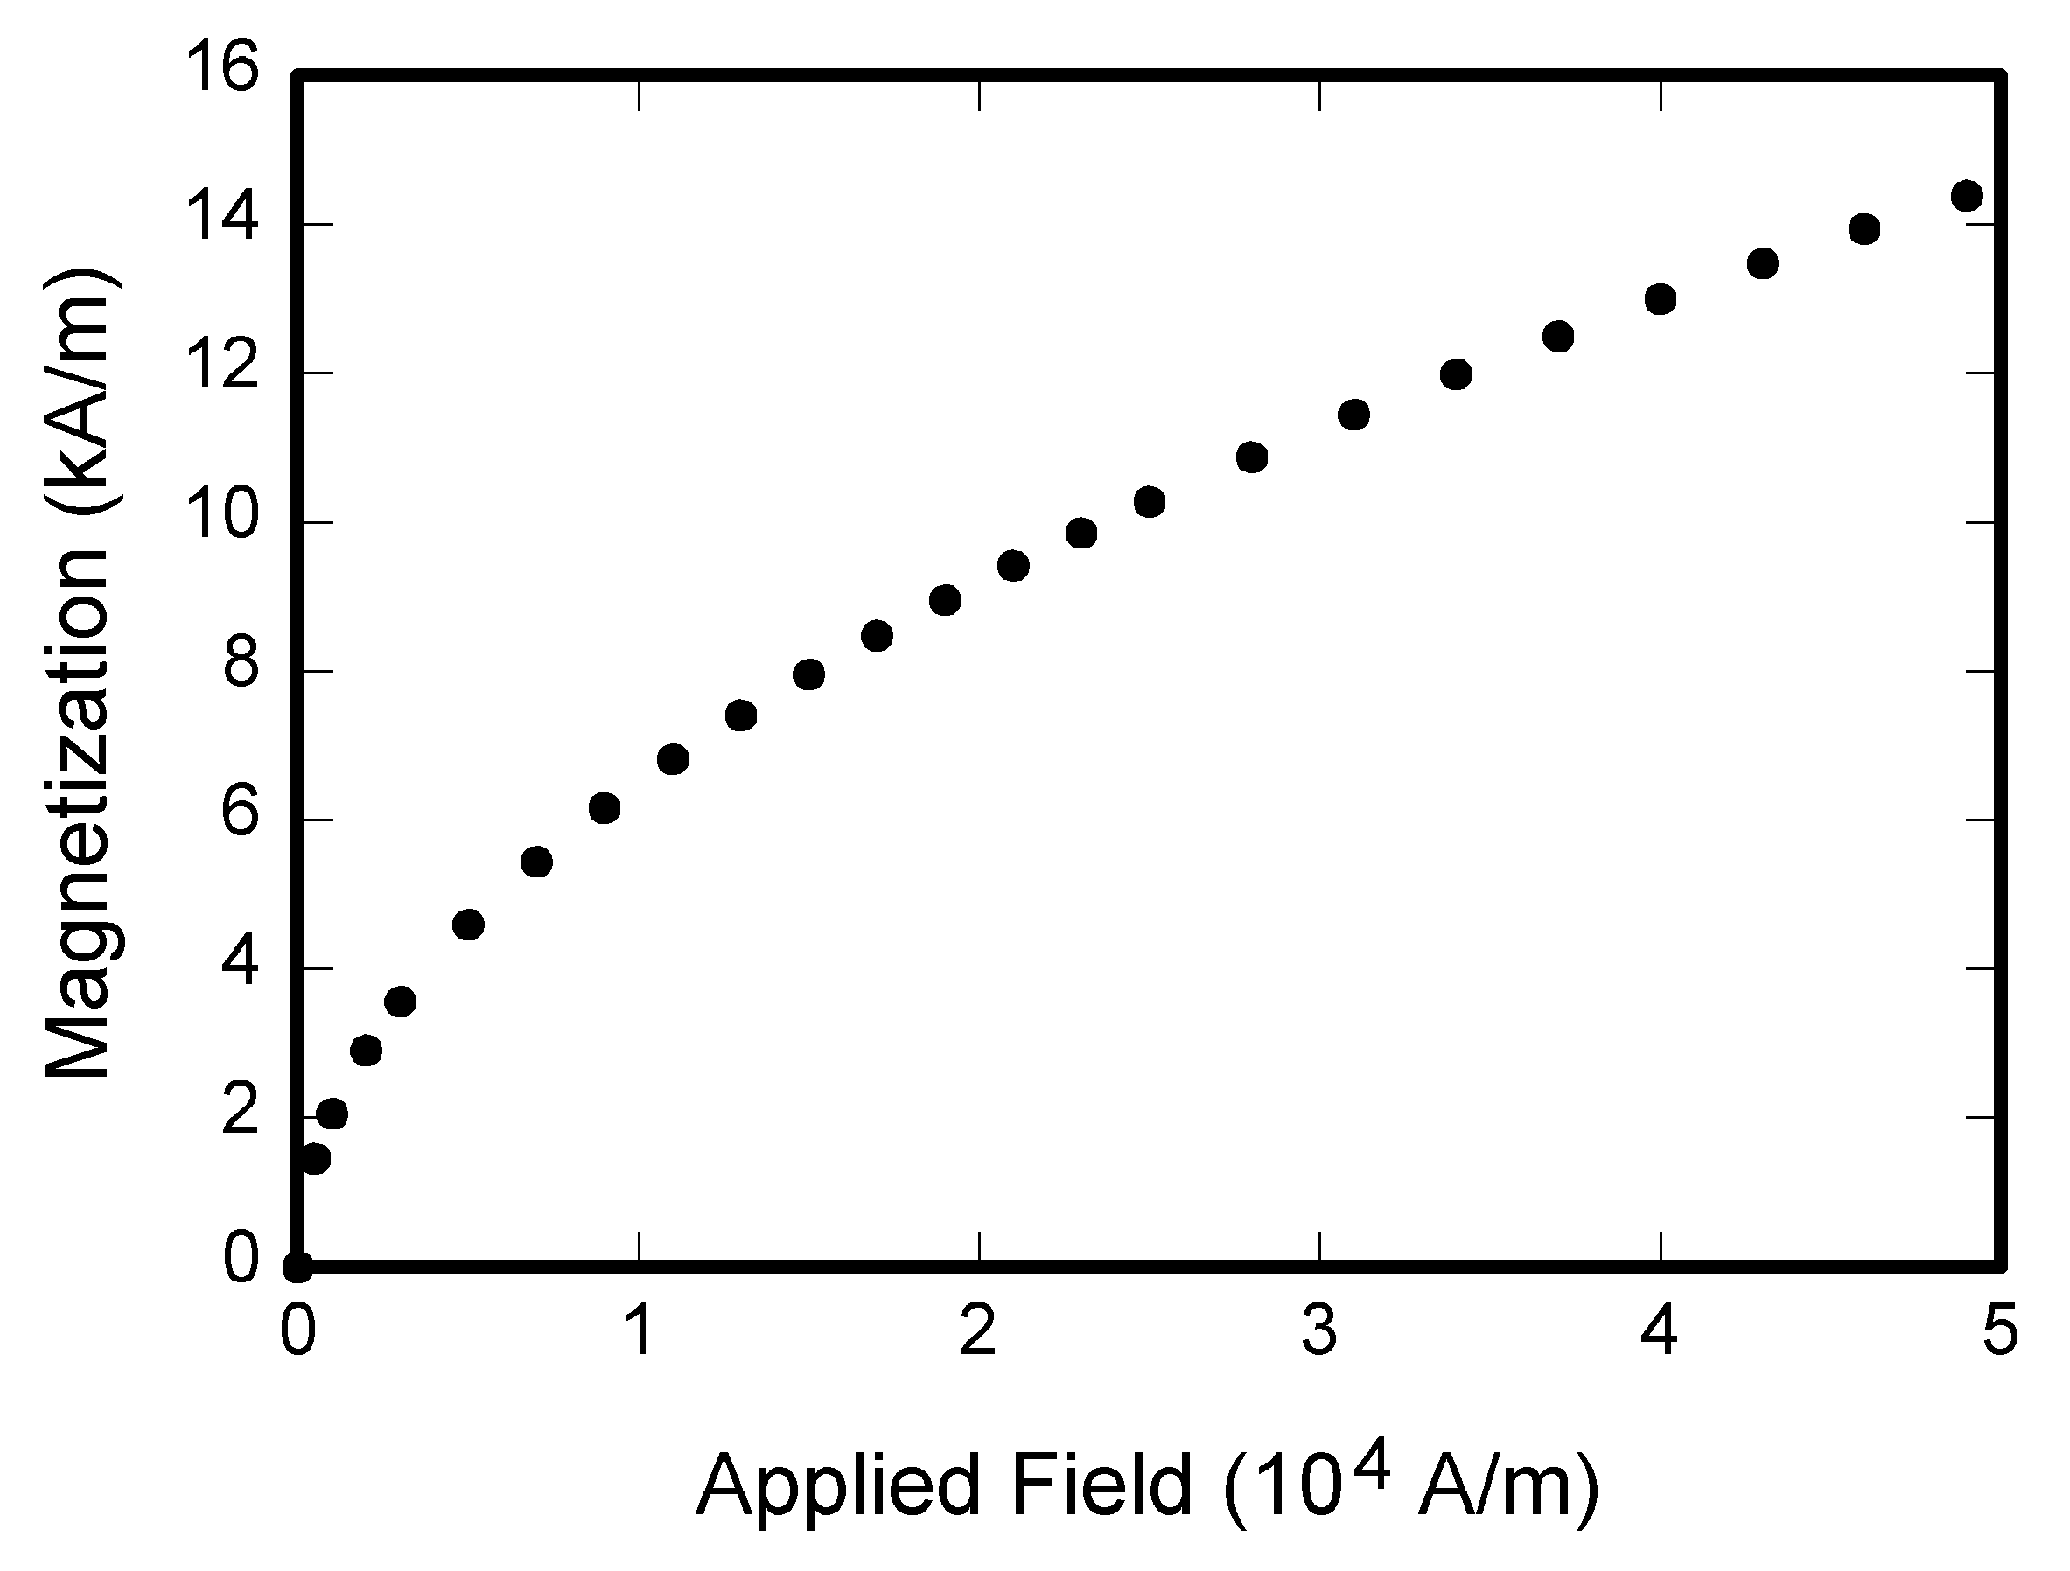
\includegraphics{fig1.png}}
% \caption{Best, average, and worst fitness over 50 generations (Pot A).}
% \label{fig1}
% \end{figure}

\subsection{Fitness Component Breakdown}
% Placeholder for Fig. 2 (Fitness Component Breakdown)
% \begin{figure}[htbp]
% \centerline{\includegraphics{fig2.png}}
% \caption{Per-component fitness breakdown for the best chromosome (Pot A).}
% \label{fig2}
% \end{figure}

Analysis across multiple pots shows a three-stage optimization process in the GA convergence. In the initial phase (typically Gens 0--15), the algorithm focuses on pruning redundant or contradictory pairwise matches. Initially, the population contains high-density chromosomes with many active pairs (e.g., 23 for Pot A) that often include contradictory geometric constraints. These contradictions lead to large Edge Residual Penalties as the BFS-based assembly construction cannot satisfy the divergent transforms. As the GA learns to deactivate these problematic genes, reducing the active pairs to a consistent subset, the residual penalty drops significantly. Simultaneously, the Cycle Penalty is typically eliminated early (e.g., by Gen 14 for Pot A), establishing a topologically consistent search space.

In the middle phase (Gens 15--35+), the best fitness often enters a refinement plateau (e.g., near $-517$ for Pot A or $+28$ for Pot F), where the algorithm explores different match combinations while keeping residuals low. This corresponds to the discovery of plausible but partially incorrect assemblies. Finally, in the late phase, successful runs exhibit a breakout from this local optimum (occurring at Gen 35 for Pot A and as late as Gen 43 for Pot F), further reducing residuals and overlaps to reach the ground-truth reconstruction. Failure cases (e.g., Pot B) typically stall in the middle-phase plateau and fail to achieve this final breakout.

\subsection{Structural Evolution}
% Placeholder for Fig. 3 (Structural Metrics)
% \begin{figure}[htbp]
% \centerline{\includegraphics{fig3.png}}
% \caption{Structural metrics for Pot A over 50 generations.}
% \label{fig3}
% \end{figure}

Structural metrics show the topological changes in the best-performing assembly over generations. Active pairs for individuals in the GA drop from 24 down to 10 to avoid contradictory pairwise matches which consequently gives a higher fitness reward.

\subsection{Visual Reconstruction Progression}
% Placeholder for Fig. 4 (Visual Progression Pot A)
% \begin{figure}[htbp]
% \centerline{\includegraphics{fig4.png}}
% \caption{Visual progression of the GA reconstruction process for Pot A.}
% \label{fig4}
% \end{figure}

The algorithm traverses through plausible but incorrect false positive configurations before escaping the local optimum to reach the perfect ground-truth reconstruction.

\subsection{Ablation Study}
Table \ref{tab4} presents results from our fitness component ablation on Pot A, where each component is disabled individually while all others remain active.

\begin{table}[htbp]
\caption{Fitness Component Ablation Study (Pot A)}
\begin{center}
\begin{tabular}{|l|c|c|c|}
\hline
\textbf{Configuration} & \textbf{Sherd \%} & \textbf{Edge \%} & \textbf{$\Delta$ Edge} \\
\hline
All components (full) & 100.0 & 100.0 & baseline \\
No inlier reward & 100.0 & 60.0 & -6 \\
No connectivity reward & 100.0 & 100.0 & 0 \\
No cycle penalty & 75.0 & 60.0 & -6 \\
No trans. residual & 100.0 & 46.7 & -8 \\
No rot. residual & 62.5 & 33.3 & -10 \\
No overlap penalty & 62.5 & 46.7 & -8 \\
Inlier reward only & 100.0 & 66.7 & -5 \\
\hline
\end{tabular}
\label{tab4}
\end{center}
\end{table}

The ablation results for Pot A show the relative importance of each fitness component. The Rotation Residual and Overlap Penalty emerged as the most critical factors; disabling them led to the largest drops in Edge Accuracy (-10 and -8 edges respectively) and a collapse in Sherd Accuracy to 62.5\%. This shows that precise rotational alignment and physical non-overlap are the primary drivers of a globally consistent assembly.

Disabling the Cycle Penalty or the Inlier Reward also significantly degraded the reconstruction, reducing Edge Accuracy to 60.0\%. This confirms that both high-quality local surface matches and global topological consistency are required to reach the ground-truth state. Interestingly, the Connectivity Reward had no impact on Pot A’s final result, suggesting that for this specific geometry, the cycle and overlap constraints were sufficient to enforce a single connected component. Finally, the Inlier Reward Only configuration achieved only 66.7\% EA, proving that while pairwise matching provides a strong starting point, global fitness optimization is essential to resolve the remaining combinatorial ambiguity.

\section{Discussion}
\subsection{False Positives vs. Bad Reconstructions}
A key challenge in designing the fitness function is distinguishing between a geometrically valid reconstruction and the true archaeological reconstruction. The fitness function evaluates local geometric consistency, such as match quality, cycle closure, edge residuals, and physical overlap, but lacks awareness of the expected global shape of the vessel.

In cases with lower Edge Accuracy such as Pot B, G, H, and J, the primary failure mode is not a visually coherent false positive, but rather bad reconstructions. In these cases, the algorithm places sherds in physically implausible or chaotic arrangements where sherds hover over each other, fail to connect cleanly, or overlap despite the penalty.

However, in other cases, the GA converges to an assembly that produces no overlap, no disagreements in residuals, and strong connectivity, yielding a high fitness score, but the shape is incorrect to a human observer expecting symmetry. We define these as false positives. For example, a false positive reconstruction of Pot F (using an alternative seed) shows sherds connected in a geometrically plausible way that is nevertheless incorrect.

This false positive phenomenon is also observable during the progression of a successful run. For instance, in the reconstruction of Pot A, the algorithm constructs a plausible but false positive partial assembly around generation 30, before successfully breaking out of the local optimum to find the true ground-truth configuration by generation 50. Since the fitness function does not encode any prior about the expected vessel profile or global symmetry, resolving false positives purely via pairwise constraints remains a limitation.

\subsection{Overlap Penalty Effectiveness}
The overlap penalty successfully reduces interpenetration artifacts in the decoded assembly. By precomputing voxel-downsampled collision clouds and using kd-tree nearest-neighbor queries, the algorithm achieves sufficient collision detection coverage at manageable computational cost. The penalty formulation efficiently bounds the penalty to avoid destabilizing the overall fitness score, while distinguishing legitimate edge contact from physical interpenetration.

\subsection{Computational Cost}
GA fitness evaluation involves BFS pose propagation, cycle penalty computation ($O(n^3)$ in sherd count), and overlap detection ($O(n^2|V| \log |V|)$), where $|V|$ is the number of points in the voxel-downsampled collision cloud. With $n = 4$ sherds, per-chromosome evaluation is extremely fast. With a population of 100 and 50 generations, total runtime remains highly competitive even on standard laptops. Though, for more complex pots like Pot D, the runtime is still too computationally expansive and need more computation to parallelize the GA even more.

\subsection{Limitations and Future Work}
One primary limitation of the current approach is that it treats reassembly as a single global optimization task, attempting to fit all sherds simultaneously. This can be difficult to achieve as the search space grows. Future work could explore a hierarchical GA strategy: performing initial iterations with smaller populations and generations to find multiple optimal partial assemblies for individual sherds, and then using these as building blocks for subsequent GA rounds. This would combine the exploratory advantages of genetic search with a structured, step-by-step construction process.

Another significant limitation is the lack of a global vessel profile prior, which often leads to geometrically valid but archaeologically incorrect false positives. Future iterations of the GA should incorporate features that evaluate whether a proposed assembly is physically plausible according to the expected vessel shape. Integrating such symmetry and profile constraints would help the algorithm differentiate between the global ground truth and local geometric local optima.

\section{Conclusion}
This paper presented a genetic algorithm-based system for the 3D reassembly of axially symmetric pottery. By replacing greedy search strategies with a population-based evolutionary approach, we successfully reconstructed two pots from the SfS++ benchmark and achieved results comparable to state-of-the-art beam search on Pot F. However, for the remaining complex vessels in the dataset, our current GA implementation lagged behind existing state-of-the-art methods. Our analysis revealed a characteristic three-stage optimization process, where the GA first prunes contradictory pairwise matches before entering a refinement plateau and finally breaking out into the ground-truth configuration.

Ablation studies confirmed that global geometric consistency, specifically enforced by rotation residual and overlap penalties, is essential for resolving the inherent ambiguity of featureless pottery fragments. While the system demonstrated strong performance on moderate datasets, challenges remain for complex vessels with high fragment counts. Future work will focus on implementing a hierarchical GA framework to build assemblies incrementally and integrating global vessel profile priors to eliminate false positive reconstructions. This work establishes evolutionary computation as a promising direction for solving large-scale combinatorial problems in archaeological restoration.

\begin{thebibliography}{00}
\bibitem{b1} J. Lu, Y. Liang, H. Han, J. Hua, J. Jiang, X. Li, and Q. Huang, ``A survey on computational solutions for reconstructing complete objects by reassembling their fractured parts,'' 2025. [Online]. Available: https://arxiv.org/abs/2410.14770
\bibitem{b2} S. J. Yoo, S. Liu, M. Z. Arshad, J. Kim, Y. M. Kim, Y. Aloimonos, C. Fermuller, K. Joo, J. Kim, and J. H. Hong, ``Structure-from-sherds++: Robust incremental 3d reassembly of axially symmetric pots from unordered and mixed fragment collections,'' 2025. [Online]. Available: https://arxiv.org/abs/2502.13986
\bibitem{b3} N. Rasheed and M. J. Nordin, ``A survey of computer methods in reconstruction of 3d archaeological pottery objects,'' International Journal of Advanced Research, vol. 3, pp. 712--714, 01 2015.
\bibitem{b4} Q.-X. Huang, S. Flory, N. Gelfand, M. Hofer, and H. Pottmann, ``Reassembling fractured objects by geometric matching,'' ACM Trans. Graph., vol. 25, no. 3, p. 569--578, Jul. 2006. [Online]. Available: https://doi.org/10.1145/1141911.1141925
\bibitem{b5} S. Winkelbach and F. M. Wahl, ``Pairwise matching of 3d fragments using cluster trees,'' International Journal of Computer Vision, vol. 78, no. 1, pp. 1--13, Jun. 2008. [Online]. Available: https://link.springer.com/article/10.1007/s11263-007-0121-5
\bibitem{b6} G. Papaioannou, T. Schreck, A. Andreadis, P. Mavridis, R. Gregor, I. Sipiran, and K. Vardis, ``From reassembly to object completion: A complete systems pipeline,'' J. Comput. Cult. Herit., vol. 10, no. 2, Mar. 2017. [Online]. Available: https://doi.org/10.1145/3009905
\bibitem{b7} R. Gregor, I. Sipiran, G. Papaioannou, T. Schreck, A. Andreadis, and P. Mavridis, ``Towards automated 3d reconstruction of defective cultural heritage objects,'' in Eurographics Workshop on Graphics and Cultural Heritage, 2014. [Online]. Available: https://api.semanticscholar.org/CorpusID:17749630
\bibitem{b8} R. Pintus, K. Pal, Y. Yang, T. Weyrich, E. Gobbetti, and H. Rushmeier, ``A survey of geometric analysis in cultural heritage,'' Computer Graphics Forum, vol. 35, no. 1, pp. 4--31, 2016. [Online]. Available: http://reality.cs.ucl.ac.uk/courses/gchstargeomanalys2014/pintus2016survey-lowres.pdf
\bibitem{b9} M. F. C. Pinho, G. L. A. Mota, and G. A. O. P. da Costa, ``A deep learning approach to assist in pottery reconstruction from its sherds,'' Heritage, vol. 8, no. 5, 2025. [Online]. Available: https://www.mdpi.com/2571-9408/8/5/167
\bibitem{b10} D. Sholomon, O. David, and N. S. Netanyahu, ``A genetic algorithm-based solver for very large jigsaw puzzles,'' in 2013 IEEE Conference on Computer Vision and Pattern Recognition. IEEE, Jun. 2013, p. 1767--1774. [Online]. Available: http://dx.doi.org/10.1109/CVPR.2013.231
\bibitem{b11} D. Sholomon, O. E. David, and N. S. Netanyahu, ``Genetic algorithm-based solver for very large multiple jigsaw puzzles of unknown dimensions and piece orientation,'' in Proceedings of the 2014 Annual Conference on Genetic and Evolutionary Computation, ser. GECCO '14. ACM, Jul. 2014, p. 1191--1198. [Online]. Available: http://dx.doi.org/10.1145/2576768.2598289
\bibitem{b12} E. Sizikova and T. Funkhouser, ``Wall painting reconstruction using a genetic algorithm,'' J. Comput. Cult. Herit., vol. 11, no. 1, Dec. 2017. [Online]. Available: https://doi.org/10.1145/3084547
\end{thebibliography}

\appendices
\section{In-Depth Visual Results Per Pottery}
This appendix provides detailed visual documentation for each pottery assembly evaluated in our study. For each pottery (Pot A through Pot J), we present the fitness convergence curves, the per-component fitness breakdown, and a side-by-side comparison of our final GA reconstruction against the archaeological ground truth.

\section{Ablation Study Visual Comparison}
This section provides a visual comparison of the final reconstructions for Pot A across all ablation configurations discussed in Section VI. These visuals illustrate how disabling specific fitness components leads to characteristic reconstruction failures, such as sherd interpenetration (no overlap penalty) or fragmented assemblies (no inlier reward).

\end{document}
